\documentclass[10pt,twocolumn]{article}
\usepackage[letterpaper,margin=0.75in]{geometry}
\usepackage{amsmath,graphicx,booktabs,xcolor,pgfplots,caption,siunitx}
\usepackage[hidelinks]{hyperref}
\pgfplotsset{compat=1.17, every axis/.style={width=0.9\columnwidth, height=0.6\columnwidth, grid=major, grid style={gray!25},
  tick label style={font=\scriptsize}, label style={font=\small}, legend style={font=\scriptsize, draw=none, fill=white, fill opacity=0.8, text opacity=1}}}
\captionsetup{font=small}
\raggedbottom
\sisetup{detect-all}
\title{\textbf{Design and Analysis of a 1\,m RC Beach Catamaran\\ with a Hydrofoil Option}}
\author{Filip Maleev\\ \small Colorado College, Department of Mathematics and Computer Science}
\date{September 2026}
\begin{document}
\maketitle

\begin{abstract}
This paper describes the design of a 1\,m radio-controlled catamaran with a beach-cat rig, two appendage configurations (daggerboards, or L-foils with T-foil rudder elevators), and a simplified 0.6\,m version intended as a first build. The hulls are 3D-printed PETG shells with bonded bulkheads, so every printed segment is a sealed compartment. The rig follows full-size beach cats: a square-top, fully battened main on a rotating wing mast, and a jib on a forestay bridle. It is modelled parametrically in Autodesk Fusion, and a custom add-in trims it with three sliders (jib sheet, main traveler, mainsheet tension). Performance is estimated with a purpose-written velocity prediction program. It combines ITTC-57 friction, Michell thin-ship wave resistance with catamaran interference (validated on the Wigley hull), appendage and foil drag, and a depowering sail model. The displacement version reaches 2.7\,m/s on a beam reach in 8\,kn of wind. Its rudders need at most 2.6$^\circ$ of an available $\pm$18$^\circ$. The foiling version reaches its 1.99\,m/s take-off speed from about 7.1\,kn of true wind, and a sensitivity study places take-off between 6.75 and 8.75\,kn. A controllability analysis shows that the foiling version is pitch-stable but has no heave stability with fixed-incidence foils: at 4\,m/s the foils lift 78\,\% more than the boat's weight. It therefore needs ride-height control. A wand-driven trailing-edge flap is sized here: it makes heave stable and well damped ($\zeta=1.4$) while using at most 13.0$^\circ$ of flap from take-off to 5\,m/s. This result led to building the non-foiling version first, preceded by a costed 0.6\,m version (\$257.37 in parts). A flight simulator built on the same physics, extended with the boat's trim in heave and pitch, then searched 306{,}180 foil designs. At speed the sail drive's bow-down couple makes the elevators push down. With a fixed positive incidence they do so by pitching the boat nose-down until they leave the water, so neither the original foils nor a first optimized set would fly. The adopted v2.2 foils set the elevators at $-1^\circ$ and 13\,mm lower, and reach 4.65\,m/s on a beam reach in 12\,kn of wind with the boat level.
\end{abstract}

\section{Introduction}
Beach catamarans such as the Hobie~16 and the Olympic Nacra~17 combine two slender hulls, a large, fully battened rig and, on the Nacra~17, foils that lift the boat clear of the water. The goal of this project was a radio-controlled model that is faithful to that type, can be built with a desktop 3D printer and off-the-shelf RC parts, and whose behaviour can be predicted before it is built. Three questions shaped the work: (i) how closely can a 1\,m model follow full-scale rig proportions; (ii) will the foiling version actually take off before it has to be depowered; (iii) will the boat be controllable. The answers set the build order: a 0.6\,m simplified version first, then the 1\,m displacement version, with foiling deferred until ride-height control is designed.

\begin{figure}[t]
\centering
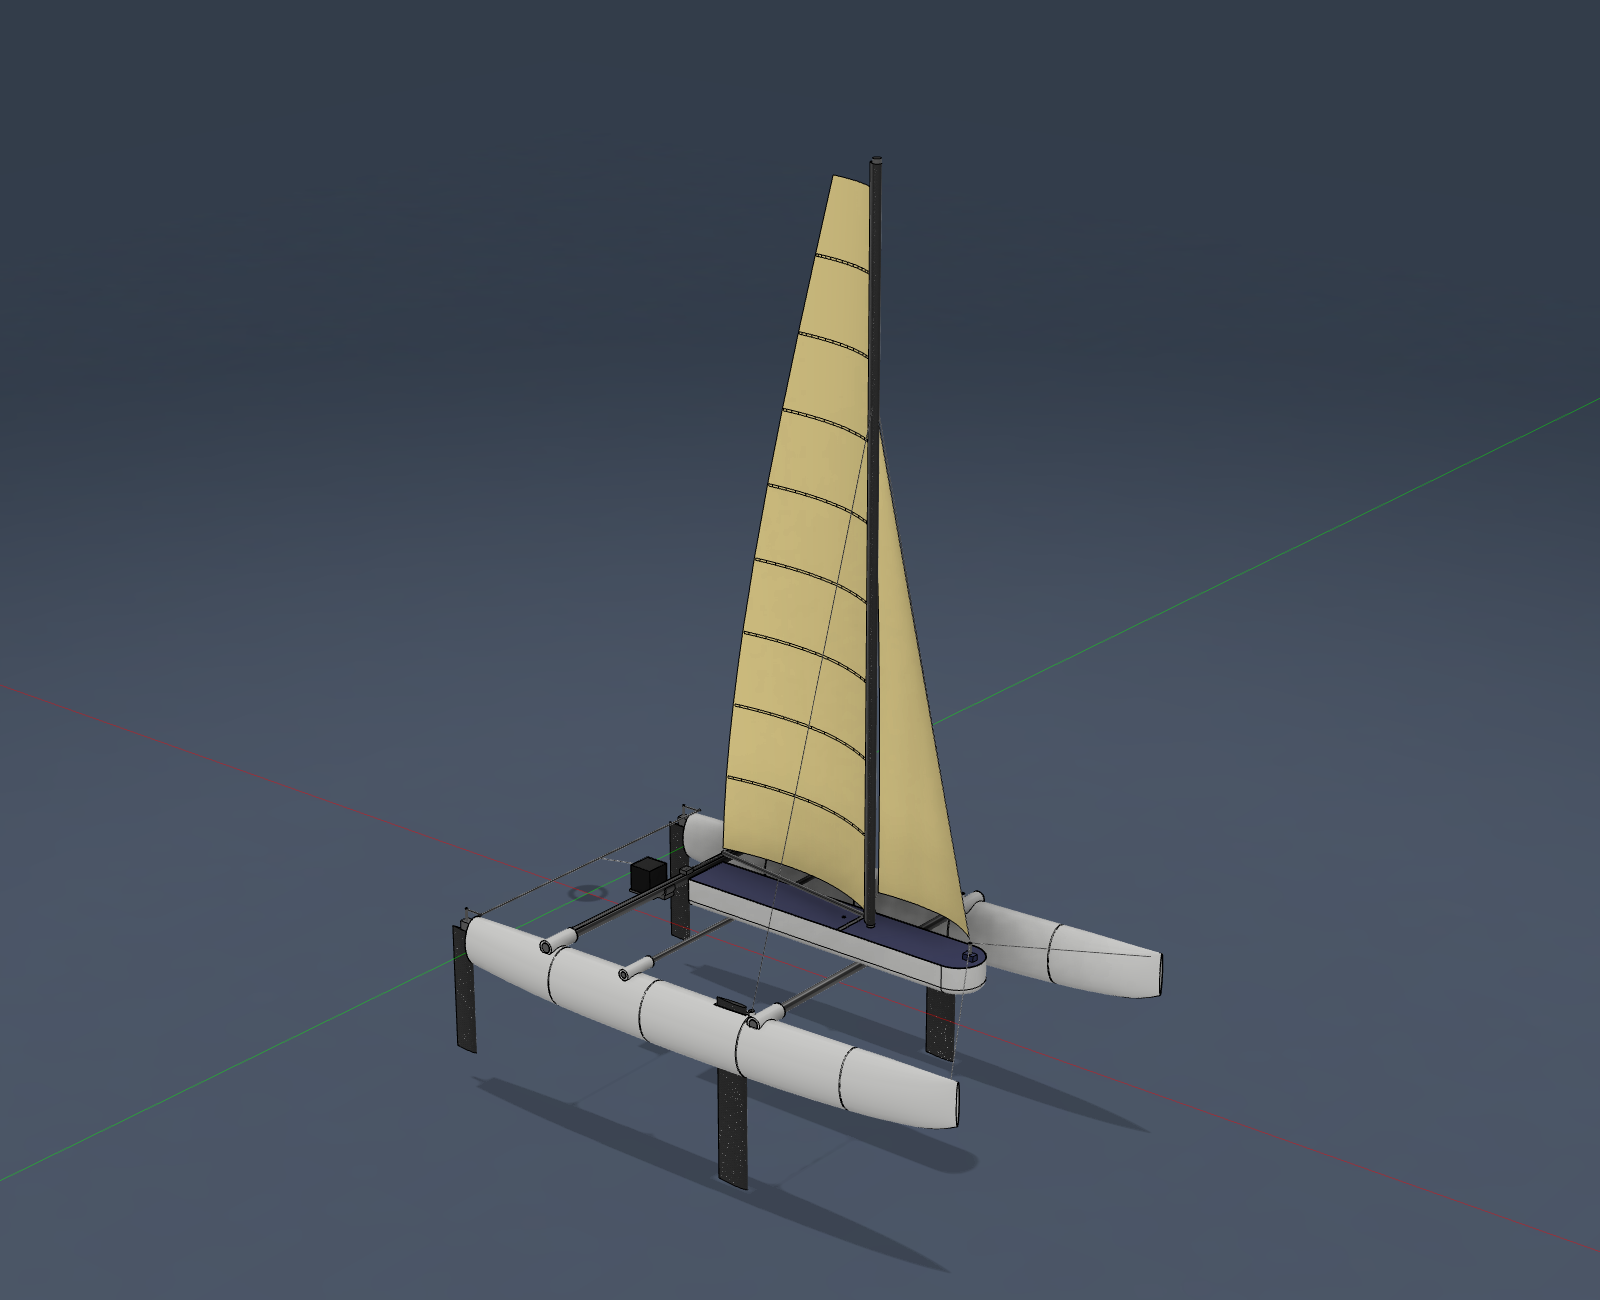
\includegraphics[width=0.49\columnwidth]{../images/build_first_v1.4.png}\hfill
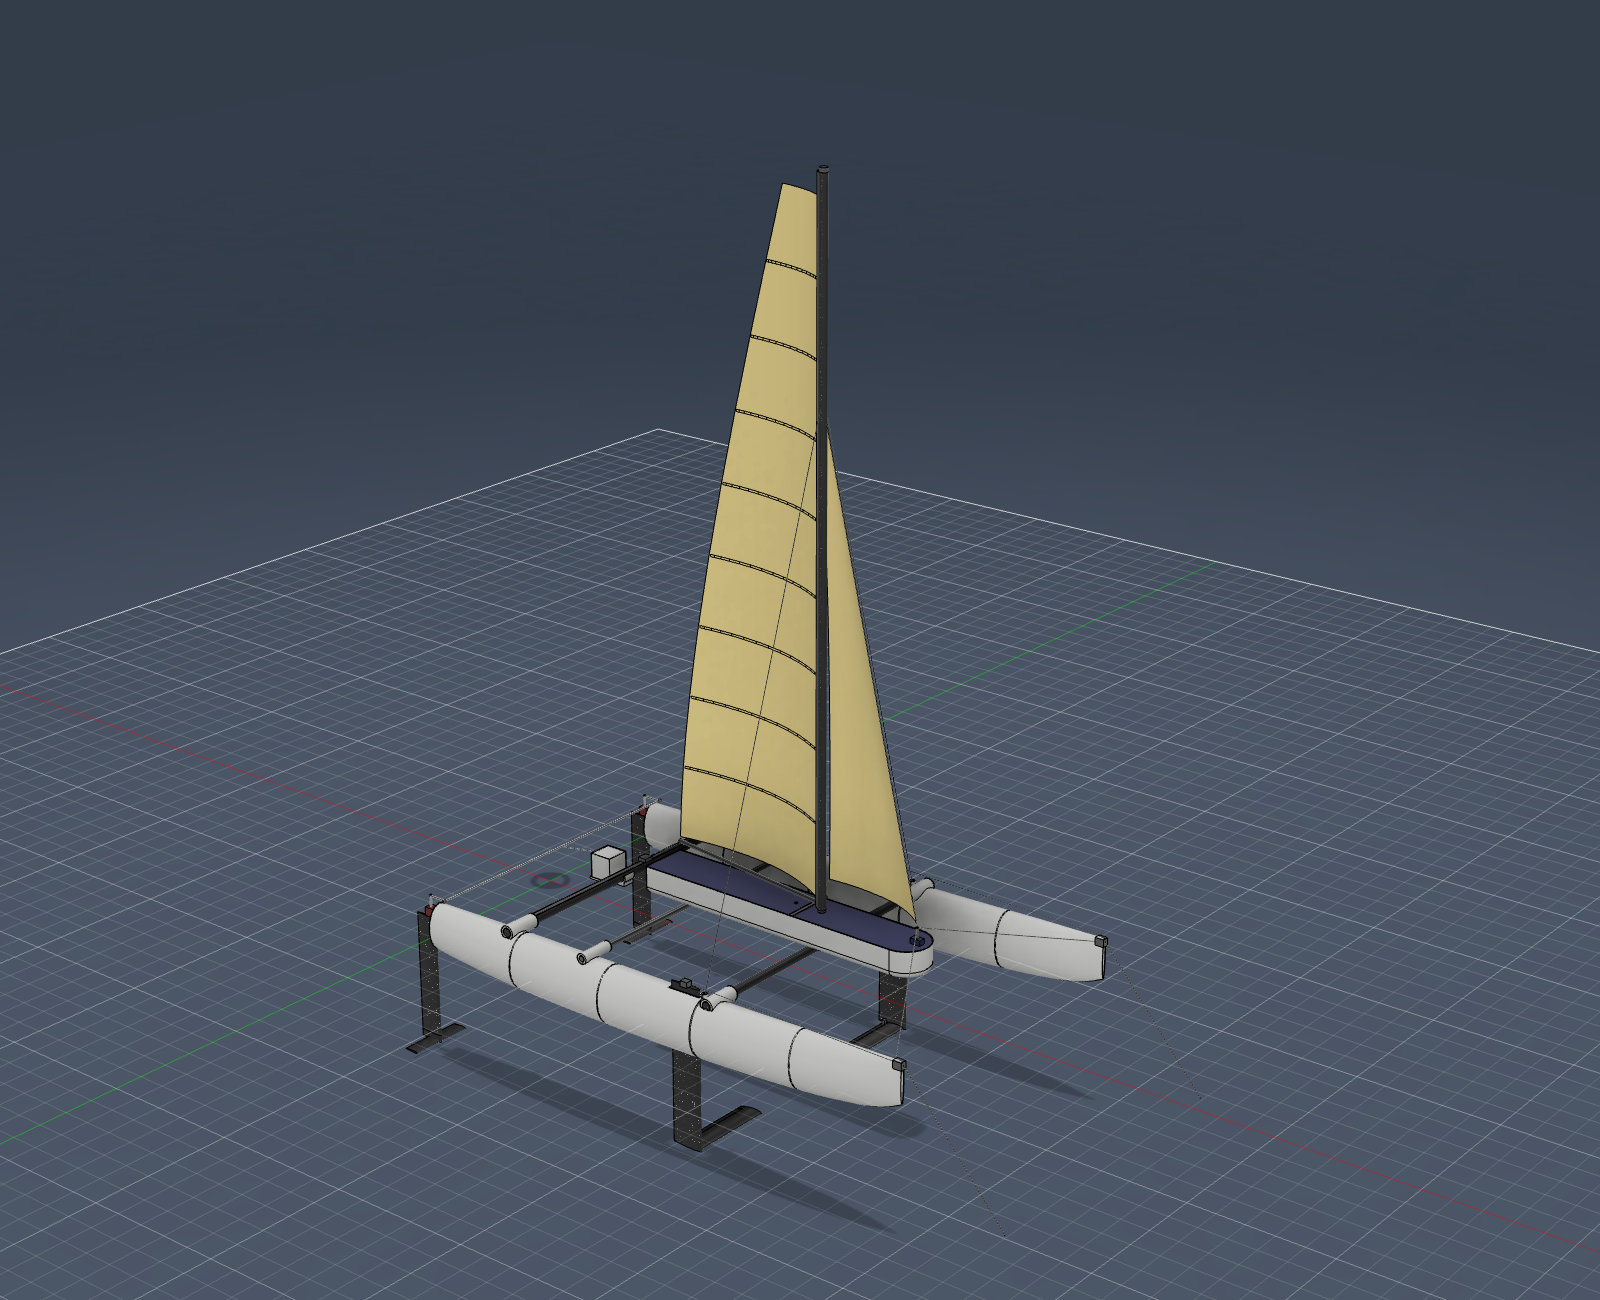
\includegraphics[width=0.49\columnwidth]{../images/foiling_v2.2.png}
\caption{The 1\,m design in Autodesk Fusion: build-first version with daggerboards (left) and foiling version with the v2.2 L-foils and T-foil rudders (right).}
\label{fig:renders}
\end{figure}

\section{Design}
\subsection{Hulls and structure}
Each hull is lofted through eight elliptical stations (Fig.~\ref{fig:plans}, right). It is 1000\,mm long, at most 80\,mm wide and 108\,mm deep, and the hull centres are 560\,mm apart. The printed hull is a 0.8\,mm PETG shell. Before shelling, 2\,mm slabs are cut from the solid loft at each print joint and bonded back in as bulkheads, so each 200\,mm segment prints as its own sealed compartment. Enclosed crossbeam sockets, foil trunks and chainplate bosses are part of the shell. The analytic hull volume from the station table matches the CAD loft to within 0.20\,\%.

\begin{figure*}[t]
\centering
\begin{tikzpicture}
\begin{axis}[name=ga, width=0.66\textwidth, height=0.62\textwidth, axis equal image, xlabel={$x$ from transom (mm)}, ylabel={$z$ (mm)}, grid=none,
  xmin=-80, xmax=1050, ymin=-280, ymax=1420, title={\small general arrangement (build-first)}]
\addplot[thick, fill=gray!15] table[x=x, y=z] {data/profile_hull.dat};
\addplot[thick, fill=blue!12] table[x=x, y=z] {data/sail_main.dat};
\addplot[thick, fill=red!12] table[x=x, y=z] {data/sail_jib.dat};
\addplot[thick, fill=black!60] table[x=x, y=z] {data/profile_board.dat};
\addplot[thick, fill=black!60] table[x=x, y=z] {data/profile_rudder.dat};
\addplot[thick, fill=blue!30] table[x=x, y=z] {data/profile_pod.dat};
\addplot[thick, fill=blue!30, unbounded coords=jump] table[x=x, y=z] {data/profile_tail.dat};
\addplot[thick, fill=gray!50] table[x=x, y=z] {data/profile_cover.dat};
\addplot[thick, fill=black, unbounded coords=jump] table[x=x, y=z] {data/profile_beams.dat};
\addplot[thin] coordinates {(259,128) (180,77)};
\addplot[very thick] coordinates {(620,72) (620,1370)};
\addplot[thick] coordinates {(603,132) (258,132)};
\addplot[thin] coordinates {(818,150) (620,1000)};
\addplot[dashed, blue] coordinates {(-80,0) (1050,0)};
\end{axis}
\begin{axis}[at={(ga.east)}, anchor=west, xshift=12mm, width=0.3\textwidth, height=0.36\textwidth, axis equal image, xlabel={$y$ (mm)}, ylabel={$z$ (mm)},
  title={\small body plan}, unbounded coords=jump, grid=none, xmin=-48, xmax=48]
\addplot[thick, blue] table[x=y, y=z] {data/bodyplan.dat};
\addplot[dashed, gray] coordinates {(-48,0) (48,0)};
\addplot[thin] coordinates {(0,-50) (0,75)};
\end{axis}
\end{tikzpicture}
\caption{Left: general arrangement of the 1\,m build-first boat (hull, the three crossbeams, pod, rudder-servo bracket and cover on the rear beam, daggerboard, rudder, rotating mast, boom and mainsheet to the traveler, square-top main and jib; dashed line: reference waterline). Right: body plan of the hull, eight elliptical stations (aft half on the left, forward half on the right).}
\label{fig:plans}
\end{figure*}

\subsection{Rig: following real beach cats}
Table~\ref{tab:rig} compares the rig with the Hobie~16 and Nacra~17 \cite{hobie,nacra}. The main-to-jib ratio (3.2) lies between the two, and the planform follows their square-top main with 8 full-length battens. The rest also comes from the full-size boats: a rotating wing mast (24\,x\,14\,mm fairing on a 12\,mm carbon tube), a forestay bridle to both bows, a traveler on the rear beam, and a jib car on a short track (on the pod lid here, because the pod sits over the front beam). Sail area and mast height, however, cannot follow geometric scaling. For a scale factor $\lambda$, righting moment scales as $\lambda^4$ (weight $\lambda^3$ times beam $\lambda$). In the same wind, the heeling moment of a similar rig scales only as $\lambda^3$ (area $\lambda^2$ times height $\lambda$). A 1:5 model with full-scale proportions would therefore be over-canvassed, so sail area was set by the VPP instead (Section~\ref{sec:results}).

\begin{table}[t]
\centering\small
\caption{Rig proportions.}
\label{tab:rig}
\begin{tabular}{lccc}
\toprule
& Hobie 16 & Nacra 17 & This boat \\
\midrule
Mast height / LOA & 1.60 & 1.71 & 1.37 \\
Main : jib area & 2.7 & 3.7 & 3.2 \\
Sail area / LOA$^2$ & 0.74 & 0.68 & 0.40 \\
\bottomrule
\end{tabular}
\end{table}

The three real-cat controls map to three RC channels and to three sliders in a Fusion add-in written for this project. Jib sheet sets the jib angle. Main traveler sets the boom angle and moves the traveler car. Mainsheet tension sets the main's twist, from $30^\circ$ loose to $3^\circ$ hard, and its depth, from 13\,\% to 8\,\%. The sails and wing mast are loft and extrude features on batten-station sketches. The add-in moves the sketch points, so the parametric model re-solves; booms, sheets and cars are updated as base-feature bodies.

\subsection{Appendages and foils}
The rudders are balanced NACA\,0012 blades (45\,mm chord, pivot at 25\,\% chord) linked by a tie bar. The build-first version has NACA\,0012 daggerboards; the foiling version replaces them with L-foils: a NACA\,0012 strut (60\,mm chord) and a NACA\,4412 wing (45\,mm chord, 160\,mm span per side) at 1.5$^\circ$ incidence. Rudder T-foil elevators (NACA\,0012, 28\,mm chord, 120\,mm span) sit at $+-1^\circ$. The foiling rudders are 13\,mm longer than the build-first ones, so the elevators sit at $z=-210$\,mm. These are the v2.2 foils chosen with the flight simulator (Section~\ref{sec:opt}). They replace the original v2.0 set (wings 200\,x\,60\,mm at $2^\circ$, elevators 150\,x\,36\,mm at $3^\circ$) and a first optimized set (v2.1) that the trim model showed would not fly. Every result in this paper is for v2.2 unless stated otherwise. An early layout placed the main foils 100\,mm deeper than the elevators. Because the elevators would breach first, that extra depth added weight and drag but no ride height, so the wings were moved up to the elevator depth, saving 73\,g of carbon.

\section{Analysis methods}
\subsection{Mass properties and hydrostatics}
Masses come from the CAD volumes, with densities or manufacturer weights for bought parts; assumptions are listed in the project README. Displacement and the centre of buoyancy are integrated over the station table with a natural cubic spline, and the flooded foil trunks are subtracted.

\subsection{Resistance}
Hull friction uses the ITTC-57 line with a form factor $(1+k)=1.25$:
\begin{equation}
R_F=\tfrac12\rho V^2 S\,C_F(1+k),\qquad C_F=\frac{0.075}{(\log_{10}Re-2)^2}.
\end{equation}
Wave resistance uses Michell's thin-ship integral \cite{michell,tuck,shipd} for a hull with half-breadth $Y(x,z)$:
\begin{equation}
R_W=\frac{4\rho g^2}{\pi U^2}\int_1^\infty \big(I^2+J^2\big)\,\frac{\lambda^2\,F_c(\lambda)}{\sqrt{\lambda^2-1}}\,d\lambda,
\end{equation}
\begin{equation}
I+iJ=\iint \frac{\partial Y}{\partial x}\,e^{\lambda^2k_0z}\,e^{i\lambda k_0x}\,dx\,dz,\qquad k_0=g/U^2,
\end{equation}
where $F_c=4\cos^2\!\big(k_0\lambda\sqrt{\lambda^2-1}\,s/2\big)$ accounts for interference between hulls a distance $s$ apart ($F_c=1$ for a single hull). The substitution $\lambda=\cosh u$ removes the endpoint singularity. $\partial Y/\partial x$ is taken as constant on each panel, and the exponential factors are integrated exactly in $x$ and $z$ (a Filon-type rule), which keeps the integral accurate at low Froude numbers. The integration was checked on the Wigley parabolic hull ($L/B=10$, $L/T=16$, Fig.~\ref{fig:wigley}): doubling the grid changes $C_W$ by less than 0.03\,\%, and the curve shows the expected hump-and-hollow shape. Thin-ship theory is reported to over-predict near the main hump \cite{tuck}, so wave drag here is, if anything, pessimistic. A transom term follows Holtrop and Mennen \cite{holtrop}. Appendage profile drag uses the ITTC line with Hoerner's thickness factor $1+2t/c+60(t/c)^4$ and a spray term $0.24\,q\,t^2$ \cite{hoerner}. Induced drag is $D_i=L^2/(q\pi e b^2)$, applied both to foil lift and to the side force carried by boards and rudders.

\begin{figure}[t]
\centering
\begin{tikzpicture}
\begin{axis}[xlabel={Froude number $Fn$}, ylabel={$10^3\,C_W$}, ymin=0]
\addplot[thick, blue] table[x=Fn, y=Cw] {data/wigley.dat};
\end{axis}
\end{tikzpicture}
\caption{Michell wave-resistance coefficient of the Wigley hull from this project's code (grid-converged to 0.03\,\%).}
\label{fig:wigley}
\end{figure}

\subsection{Foils and sails}
Foil lift uses the thin-airfoil zero-lift angle, $\alpha_{L0}=-\frac1\pi\int_0^\pi \frac{dy_c}{dx}(\cos\theta-1)\,d\theta = -4.15^\circ$ for NACA\,4412, and the lifting-line slope $a=2\pi/(1+2/(e\,AR))$ with $e=0.85$ \cite{anderson}. The sails produce $F_x=q_aA(C_L\sin\beta-C_D\cos\beta)$ (drive) and $F_y=q_aA(C_L\cos\beta+C_D\sin\beta)$ (heel), with $C_D=C_{D0}+C_L^2/(\pi e_sAR_s)$, $C_{L,\max}=1.3$ and $C_{D0}=0.05$. $C_L$ is reduced (the sails are flattened) whenever $F_yh$ would exceed 90\,\% of the maximum righting moment $W s/2$. The sails are also eased (both forces scaled down) whenever the bow-down moment $F_xh_p$ would exceed 90\,\% of the largest longitudinal righting moment the hulls can provide (Section~\ref{sec:stab}); $h_p$ is measured from the centre of effort to the hull resistance centre. Beyond a beam reach the model blends to a stalled sail ($C_D\to1.2$). The VPP marches boat speed up from rest until drive equals drag; for the foiling version it switches to the flying branch once both foils can carry their share of the weight. Below take-off the wand holds the flaps fully down, so the main foils' lift (and its induced drag) uses the full $15^\circ$ of flap (Section~\ref{sec:rh}). Every foil lift coefficient is capped at 0.8, i.e. 0.8 of an assumed section maximum of 1.0 near $Re=10^5$.

\subsection{Flying trim in heave and pitch}\label{sec:trim}
Once flying, the foils must carry the weight and also balance the pitching moment. The sail drive $F$ equals the flying drag. It acts at the sail centre of effort, while the drag acts at the appendages, so the boat feels a bow-down couple $M=F\,(z_{CE}-z_D)$, with $z_D$ the drag-weighted height of the appendage forces. Moment balance about the centre of gravity gives the foil loads
\begin{equation}
L_e=\frac{W a-M}{a+c},\qquad L_m=W-L_e,
\end{equation}
where $a$ and $c$ are the distances from the CG to the main-foil and elevator quarter chords. The couple moves load from the elevators to the main foils, and at speed the elevators must push down. The fixed-incidence elevators then set the pitch, $\theta=L_e/(qS_ea_e)-i_e$, and the wand-driven flaps make up the main foils' lift. The wand is hinged at the bow with its tip on the water, and its angle is read in the boat frame, so the bow height is $h_p=L\sin(\phi_0-\delta/G-\theta)$. The depth of every appendage follows from $h_p$ and $\theta$, and the strut and rudder drag use those immersed lengths. A speed belongs to the flying range when:
\begin{itemize}\itemsep1pt
\item both foils stay within the usable lift coefficient and the flaps within $\pm15^\circ$;
\item the main foils and elevators stay at least half a chord deep;
\item at least 30\,mm of rudder stays in the water (an assumed immersion limit);
\item the rudders, at their trimmed immersion, can hold the largest side force the sails can apply before the boat heels out, using at most 80\,\% of their $\pm18^\circ$ throw (the reserve is assumed);
\item the hulls stay clear.
\end{itemize}
Take-off is the lowest such speed. Above the range the sails must be eased, and the VPP caps the speed there.

\subsection{Controllability}
Steady yaw balance requires the rudders to cancel $M=F_y(x_{CE}-x_{CLR})+R_{\text{hull}}\,u\,s/2$, where $u$ is the fraction of righting moment in use; the second term is the extra drag of the loaded leeward hull. The rudder force $F_r=M/(x_{CLR}-x_r)$ is converted to a rudder angle with the lifting-line slope, and the windward rudder is taken as clear of the water for $u>0.8$. Foil pitch stability uses the neutral point $x_{np}=(a_mS_mx_m+\eta a_eS_ex_e)/(a_mS_m+\eta a_eS_e)$ with $\eta=1$ or $0.65$ to bracket downwash on the elevators.

\section{Results}\label{sec:results}
\subsection{Mass and hydrostatics}
\begin{table}[t]
\centering\small
\caption{Mass properties and hydrostatics.}
\label{tab:hydro}
\resizebox{\columnwidth}{!}{\begin{tabular}{lccc}
\toprule
& 1\,m build-first & 1\,m foiling & 0.6\,m mini \\
\midrule
Mass (g) & 2037 & 2242 & 755 \\
Hull draft (mm) & 28.6 & 29.9 & 23.8 \\
LCG / LCB (mm) & 457 / 431 & 462 / 432 & 258 / 262 \\
One-hull buoyancy / weight & 2.74 & 2.49 & 2.05 \\
Max righting moment (N\,m) & 5.60 & 6.16 & 1.26 \\
Sail area (m$^2$) & 0.401 & 0.401 & 0.144 \\
\bottomrule
\end{tabular}}
\end{table}
Table~\ref{tab:hydro} lists the three boats. The heaviest items on the 1\,m build-first boat are the hulls (783\,g), the centre pod (336\,g) and the RC electronics (313\,g); the foiling kit adds 376\,g. The design target was that one hull alone could float at least twice the boat's weight; all three versions meet it.

\subsection{Resistance and speed}
\begin{figure}[t]
\centering
\begin{tikzpicture}
\begin{axis}[xlabel={Boat speed $V$ (m/s)}, ylabel={Resistance (N)}, legend pos=north west, ymin=0]
\addplot[thick, blue] table[x=V, y=R] {data/resistance_displacement.dat}; \addlegendentry{build-first (total)}
\addplot[thick, red] table[x=V, y=R] {data/resistance_foiling.dat}; \addlegendentry{foiling (total)}
\addplot[dashed, blue] table[x=V, y=wave] {data/resistance_displacement.dat}; \addlegendentry{build-first wave (Michell)}
\addplot[dotted, thick, blue] table[x=V, y=fric] {data/resistance_displacement.dat}; \addlegendentry{build-first hull friction}
\end{axis}
\end{tikzpicture}
\caption{Resistance at zero side force. The foiling curve peaks just before take-off (1.99\,m/s) and drops once the hulls leave the water.}
\label{fig:res}
\end{figure}

\begin{figure}[t]
\centering
\begin{tikzpicture}
\begin{axis}[xlabel={True wind speed (kn)}, ylabel={Boat speed (m/s)}, legend pos=north west, ymin=0, xmin=3, xmax=16, ymax=6.2]
\addplot[thick, blue, mark=*, mark size=1pt] table[x=tws, y=V] {data/vpp_displacement_90.dat}; \addlegendentry{build-first, TWA 90$^\circ$}
\addplot[thick, blue, dashed] table[x=tws, y=V] {data/vpp_displacement_60.dat}; \addlegendentry{build-first, TWA 60$^\circ$}
\addplot[thick, red, mark=square*, mark size=1pt] table[x=tws, y=V] {data/vpp_foiling_90.dat}; \addlegendentry{foiling, TWA 90$^\circ$}
\addplot[thick, red, dashed] table[x=tws, y=V] {data/vpp_foiling_60.dat}; \addlegendentry{foiling, TWA 60$^\circ$}
\end{axis}
\end{tikzpicture}
\caption{Predicted boat speed. The jump in the foiling curves is take-off. The build-first boat must depower above about 8--9\,kn.}
\label{fig:vpp}
\end{figure}

Figures~\ref{fig:res} and~\ref{fig:vpp} show the predicted resistance and speed. Hull friction and appendage drag dominate the build-first boat; Michell wave drag stays below 0.42\,N up to 3\,m/s because the hulls are slender ($L/B=12.5$). Below take-off, the foils cost the foiling version 25--26\,\% of its speed. The foiling version takes off from about 7.1\,kn of true wind, which is below the 8--9\,kn where the rig starts to depower, so a usable foiling window exists. Table~\ref{tab:sens} shows that this conclusion holds across the least certain inputs.

\begin{table}[t]
\centering\small
\caption{Take-off speed and the lowest true wind (kn) at which the foiling version takes off.}
\label{tab:sens}
\resizebox{\columnwidth}{!}{\begin{tabular}{lccc}
\toprule
Scenario & $V_{to}$ (m/s) & TWA 60$^\circ$ & TWA 90$^\circ$ \\
\midrule
baseline & 1.99 & 7.75 & 7.25 \\
sail CLmax 1.1 & 1.99 & 8.25 & 7.75 \\
sail CLmax 1.5 & 1.99 & 7.25 & 6.75 \\
foil lift -20\% (low Re, free surface) & 2.16 & 7.75 & 7.5 \\
mass +10\% & 2.09 & 8.0 & 7.5 \\
mass -10\% & 1.89 & 7.25 & 6.75 \\
sail-drive pitch couple x0.5 & 1.87 & 7.5 & 7.0 \\
sail-drive pitch couple x1.5 & 2.24 & 8.75 & 7.5 \\
\bottomrule
\end{tabular}}
\end{table}

\subsection{Controllability}
\textbf{Build-first version.} Over 4--14\,kn and TWA 60--105$^\circ$ the rudders need at most 2.6$^\circ$ (TWA 60$^\circ$, 8\,kn, one rudder working) of the $\pm18^\circ$ that the linkage gives. That leaves at least 78\,\% margin to stall, and the servo torque needed is below 0.09\,kg\,cm.

\noindent\textbf{Foiling version.} Steering while flying needs at most 4.4$^\circ$, with 74\,mm of rudder immersed in that case (from the flying trim). The foil system is statically pitch-stable: the CG lies 32--84\,mm ahead of the neutral point. Heave is the problem (Fig.~\ref{fig:heave}). With fixed incidence, lift grows as $V^2$ while weight is constant, so nothing sets the flying height: the boat would climb until a foil breaches and ventilates, then drop. Holding height requires the main-foil angle to change by +3.7$^\circ$ at 2\,m/s but -3.3$^\circ$ at 4\,m/s. If the boat is also free to pitch, the fixed-incidence elevators trim it nose-down as speed rises. That reduces the excess but does not remove it, and nothing still ties lift to height, so heave stays neutral. Ride-height control is therefore required before the foiling version can fly under control (Section~\ref{sec:rh}).

\begin{figure}[t]
\centering
\begin{tikzpicture}
\begin{axis}[width=0.78\columnwidth, xlabel={Boat speed (m/s)}, ylabel={Lift excess over weight (\%)}, axis y line*=left]
\addplot[thick, red, mark=*] table[x=V, y=excess] {data/heave.dat};
\end{axis}
\begin{axis}[width=0.78\columnwidth, ylabel={Foil angle change ($^\circ$)}, axis y line*=right, axis x line=none, grid=none]
\addplot[thick, blue, dashed, mark=square*] table[x=V, y=dalpha] {data/heave.dat};
\end{axis}
\end{tikzpicture}
\caption{Fixed-incidence foils: lift in excess of weight (solid, left axis) and the main-foil angle change needed to hold height (dashed, right axis).}
\label{fig:heave}
\end{figure}

\subsection{Static stability and pitchpole}\label{sec:stab}
\textbf{Heel.} The transverse righting arm (Fig.~\ref{fig:gz}) comes from clipping the heeled elliptical sections of both hulls at the waterline, with the waterline height solved so displacement equals weight. The 1\,m build-first boat reaches its largest righting arm, 271\,mm, at 6$^\circ$ of heel, when the windward hull lifts. The maximum righting moment, 5.41\,N\,m, is within 3\,\% of the $Ws/2$ used in the VPP, which confirms that assumption. The boat capsizes at about 80$^\circ$ (mini: 80$^\circ$).

\noindent\textbf{Pitchpole.} A catamaran more often trips over its bows than capsizes sideways. Tilting the waterline bow-down and re-solving the sinkage gives the largest longitudinal righting moment the hulls can provide before the bows go under: 4.77\,N\,m on both hulls and 3.64\,N\,m on one hull (the windward hull flying). Setting that equal to the sails' bow-down moment gives the wind above which the sails must be eased on each point of sail. For the 1\,m boat that is >20 / 9 / 11.5 / 16\,kn at TWA 60/90/120/150$^\circ$, and for the mini 7.5 / 8.5 / 10 / 13.5\,kn. These limits sit close to the heel limits, so pitch-limited depowering was added to the VPP.

\noindent\textbf{Design iteration: bow volume.} Table~\ref{tab:bows} compares the original hull with three variants that add volume only to the forward stations, mostly above the waterline. Variant B was adopted as the v1.3 hull. It raises the one-hull pitch limit by 23\,\% for 13\,g and a 0.4\,\% drag increase at 2\,m/s. Variant C adds little more for 50\,\% more weight.

\begin{figure}[t]
\centering
\begin{tikzpicture}
\begin{axis}[xlabel={Heel angle ($^\circ$)}, ylabel={Righting arm GZ (mm)}, legend pos=north east, xmin=0, xmax=90]
\addplot[thick, blue, mark=*, mark size=1pt] table[x=deg, y=gz] {data/gz_build_first_1m.dat}; \addlegendentry{1\,m build-first}
\addplot[thick, red, mark=square*, mark size=1pt] table[x=deg, y=gz] {data/gz_mini_600.dat}; \addlegendentry{0.6\,m mini}
\addplot[gray, dashed] coordinates {(0,0) (90,0)};
\end{axis}
\end{tikzpicture}
\caption{Transverse righting arm from the heeled hull geometry. It peaks when the windward hull lifts; the curve crosses zero at the capsize angle.}
\label{fig:gz}
\end{figure}

\begin{table}[t]
\centering\small
\caption{Bow-volume variants of the 1\,m hull (B adopted as v1.3). Pitchpole limits in kn at TWA 60/90/120$^\circ$.}
\label{tab:bows}
\resizebox{\columnwidth}{!}{
\begin{tabular}{lccccc}
\toprule
Variant & $RM_L$ 1 hull (N\,m) & $RM_L$ 2 hulls (N\,m) & Drag at 2\,m/s (N) & $\Delta m$ (g) & Pitchpole (kn) \\
\midrule
baseline & 2.92 & 4.29 & 3.514 & +0 & 9.5 / 9 / 10.5 \\
A & 3.12 & 4.32 & 3.517 & +7 & 10.5 / 9 / 11 \\
B & 3.59 & 4.72 & 3.527 & +13 & >20 / 9 / 11 \\
C & 3.96 & 4.90 & 3.535 & +20 & >20 / 9 / 11.5 \\
\bottomrule
\end{tabular}}
\end{table}

\subsection{Foil structure}
With the largest main-foil flight load, which occurs at speed when the elevators push down, all on one wing under a 2\,g gust (63.1\,N; root moment 5050\,N\,mm), the section properties computed from the NACA coordinates give the results in Table~\ref{tab:struct}. Printed PETG is strong enough but far too flexible, so the foils must be carbon. A home-buildable alternative to solid carbon is a printed core with unidirectional carbon caps (4 layers of 0.127\,mm tape, 25\,mm wide, on each face). Taking $E\approx120$\,GPa for the cap laminate (assumed), centring the caps on the thickest point and ignoring the core, the caps give 69\,\% of the solid-carbon bending stiffness: tip deflection 2.16\,mm and cap stress 122\,MPa in the load case above. The v2 foiling kit (cores, carbon tape, laminating epoxy, flap hinges, wands and linkage) costs \$99.45.
\begin{table}[t]
\centering\small
\caption{L-foil structural check (v2.2 foils).}
\label{tab:struct}
\resizebox{\columnwidth}{!}{\begin{tabular}{lccc}
\toprule
Material & Root stress & Tip deflection & Strut rotation \\
\midrule
CFRP ($E$ = 70 GPa) & 49.7 MPa & 1.49 mm & 0.82$^\circ$ \\
Printed PETG ($E$ = 2 GPa) & 49.7 MPa & 52.18 mm & 28.70$^\circ$ \\
\bottomrule
\end{tabular}}
\end{table}

\subsection{Rig and crossbeam loads}\label{sec:rigload}
The largest steady side force the sails can apply is set by the righting moment, $F = RM_{\max}/h$ with $h$ the heeling arm; beyond it the boat heels and sheds load. Carried by a mast pinned at the step and held by the windward shroud at the hounds, this force gives the shroud tension. The jib's share (by area), on a forestay with an assumed 2\,\% sag, gives the forestay tension, and the vertical components of both compress the mast. A harder case is the sheet servo at its stall torque (spec-sheet values at 4.8\,V), for example with the sheet held in against a stop. The mast is checked for Euler buckling between step and hounds. Each crossbeam is checked as a simply supported tube loaded at mid-span. On the mini, the box levers the sheet load onto both beams. Table~\ref{tab:rigload} lists the results. $E = 70$\,GPa and a bending strength of 300\,MPa are assumed for the carbon tubes, since no values are published for the tubes used.

\begin{table}[h]
\centering\small
\caption{Rig and crossbeam loads (sails at the heel limit; ``stall'' adds the sheet servo at stall torque).}
\label{tab:rigload}
\resizebox{\columnwidth}{!}{\begin{tabular}{lcc}
\toprule
 & 1\,m build-first & Mini \\
\midrule
Side force at the heel limit (N) & 8.0 & 2.9 \\
Shroud / forestay tension (N) & 16 / 12 & 5.9 / 4.3 \\
Mainsheet at servo stall (N) & 92 & 34 \\
Mast compression, sailing / stall (N) & 27 / 119 & 10 / 44 \\
Mast Euler load (N) / safety at stall & 423 / 3.6 & 107 / 2.4 \\
Front beam: MPa / mm / safety & 100 / 4.7 / 3.0 & 54 / 1.5 / 5.6 \\
Rear beam: MPa / mm / safety & 77 / 3.6 / 3.9 & 40 / 1.1 / 7.6 \\
Pod beam, 5\,g: MPa / mm / safety & 35 / 2.6 / 8.7 & -- \\
\bottomrule
\end{tabular}}
\end{table}

The sailing loads are small: the sheet servos, not the wind, set the structural load case. With its first 8\,x\,7\,mm beams (0.5\,mm wall), the mini's front beam reached a safety factor of only 2.0 in the stall case and deflected 5.2\,mm. It now uses 10\,x\,8\,mm tube, which costs \$1.05 less, for 18\,g more.

\section{Ride-height control}\label{sec:rh}
Each L-foil wing gets a trailing-edge flap of 25\,\% chord (11\,mm) from 10\,mm inside the tip to the strut, 146\,mm of the 160\,mm span. A carbon wand hinged at each bow trails on the water and drives that hull's flap through a deck pushrod, a bellcrank and a rod inside the strut. Each foil therefore regulates its own height, which also adds roll stability. Thin-airfoil theory gives the flap effectiveness
\begin{equation}
\tau = 1-\frac{\theta_h-\sin\theta_h}{\pi},\qquad \cos\theta_h = 2E-1,
\end{equation}
so $\tau=0.609$ for $E=0.25$; 0.487 is used after a 20\,\% viscous reduction. The wand is 300\,mm long at 49$^\circ$, so its angle changes by 5.08\,rad per metre of height. The linkage gearing is 1.5$^\circ$ of flap per degree of wand.

\noindent\textbf{Trim.} At each speed the elevators set the pitch and the flaps make up the main foils' lift, with the sail-drive couple included (Section~\ref{sec:trim}). From take-off at 1.99 to 5.0\,m/s the flap angle stays between $-6.7$$^\circ$ and $13.0$$^\circ$, inside the $\pm15^\circ$ travel (Fig.~\ref{fig:rh}). The boat pitches between $+0.0$$^\circ$ and $+0.4$$^\circ$ (nose up $+$), and the bow flies $-32$ to $+15$\,mm from its design height.

\noindent\textbf{Heave stability.} Linearised heave dynamics are
\begin{gather}
m\ddot h + c\,\dot h + k\,h = 0,\\
c=\frac{q(S_ma_m+S_ea_e)}{V},\qquad k=q\,S_ma_m\,\tau\,G\,\frac{d\phi}{dh},
\end{gather}
where $c$ comes from the change of foil angle of attack with vertical velocity ($\dot h/V$) and $k$ from the wand feedback. With fixed foils $k=0$, so nothing restores height. With the wand, $k$ rises from 404 to 2527\,N/m and the natural frequency from 2.1 to 5.3\,Hz. Because $c\propto V$ and $\sqrt{k}\propto V$, the damping ratio is the same at every speed, $\zeta=1.4$ (over-damped): disturbances die out without oscillating. A time-domain run of the same model (\texttt{analysis/foil\_checks.py}) confirms this: across the flying range a 20\,mm height disturbance decays to 5\,\% in 0.22--0.54\,s with no overshoot, while with fixed foils it does not decay at all. The same script checks the trim over the flying range up to the 12\,kn beam-reach speed: the elevators stay at least 1.57 chords deep, the main foils 1.20 chords, and at least 47\,mm of rudder stays in the water. At take-off, with the flaps fully down, the main foils need $C_L=0.80$. 28 of 28 foil checks pass.

\noindent\textbf{Heave and pitch together.} The wand sits a metre ahead of the elevators, so heave and pitch are coupled: the wand reads the bow height and the boat-frame angle, and each foil feels the vertical velocity of its own station, $\dot h + l\,\dot\theta$. Linearising both degrees of freedom about the trim, with the pitch inertia from the CAD model ($I_{yy}=0.207$\,kg\,m$^2$, radius of gyration 304\,mm), gives a fourth-order system (\texttt{analysis/pitch\_heave.py}). Across the flying range it is stable (Routh--Hurwitz), with one oscillating mode at 1.8--7.0\,Hz and damping ratio at least 0.64 (0.62 with an elevator efficiency of 0.65), and two non-oscillating decaying modes. That is less damping than the heave-only estimate ($\zeta=1.36$), but the motion stays well damped. With fixed foils one root sits at zero: heave stays neutral. Unsteady lift, added mass and downwash lag are left out.

\begin{figure}[t]
\centering
\begin{tikzpicture}
\begin{axis}[xlabel={Boat speed (m/s)}, ylabel={Angle ($^\circ$)}, legend pos=south west]
\addplot[thick, red] table[x=V, y=flap] {data/ride_height.dat}; \addlegendentry{flap angle}
\addplot[thick, blue, dashed] table[x=V, y=pitch] {data/ride_height.dat}; \addlegendentry{boat pitch}
\end{axis}
\end{tikzpicture}
\caption{Wand-controlled flight across the flying range: flap angle and boat pitch from the trim of Section~\ref{sec:trim}, sail-drive couple included. Flap travel is $\pm15^\circ$.}
\label{fig:rh}
\end{figure}

\section{Foil design with the flight simulator}\label{sec:opt}
The VPP answers whether a given design flies; to ask which foils fly best, it was turned into an interactive flight simulator (a web page, \texttt{sim/foil\_sim.html}). Its physics are the VPP's, including the flying trim of Section~\ref{sec:trim}: the Michell wave resistance is tabulated against boat speed and the weight the hulls carry, and every other term is computed live. At the CAD design it reproduces the Python VPP's boat speed to 0.02\,m/s in all 12 reference cases (build-first and foiling, 6--10\,kn, 60 and 90$^\circ$). It adds:
\begin{itemize}\itemsep1pt
\item foil span, chord and incidence, and the elevator height, as inputs;
\item foil and rudder mass and the resulting shift of the centre of gravity, with the densities of the CAD mass export;
\item the wand-driven flaps: fully down below take-off (they add induced drag there), then trimmed to hold ride height;
\item a cap on the usable foil lift coefficient of 0.8 (0.8 of an assumed section maximum of 1.0 near $Re=10^5$).
\end{itemize}

\noindent\textbf{A first search, and why it was withdrawn.} A first search was run before the trim model existed. It assumed each foil pair carried a fixed share of the weight at level attitude, so the elevators set the take-off speed. It recommended smaller foils with the elevators at $4^\circ$ (v2.1: wings 160\,x\,40\,mm at $0^\circ$, elevators 140\,x\,32\,mm at $4^\circ$), and these were drawn in CAD. The trim model reverses that result. At 4.5\,m/s the v2.2 foils must balance a 5.3\,N\,m bow-down couple, more than the elevators' share of the weight times the foil spacing, so the elevators must push down. Fixed at $+4^\circ$, they can only do that by pitching the whole boat nose-down. The stern, a metre behind the wand that holds the bow, then rises until the elevators leave the water: for v2.1 the elevator reaches the surface at 2.5\,m/s (Fig.~\ref{fig:trim}). Neither the original v2.0 foils nor v2.1 has any speed at which the trim is feasible: as drawn, they would not fly.

\begin{figure}[t]
\centering
\begin{tikzpicture}
\begin{axis}[width=\columnwidth, height=0.62\columnwidth, xlabel={Boat speed (m/s)}, ylabel={Elevator depth (mm)}, ymin=-60, ymax=100, xmin=2, xmax=5, legend style={font=\scriptsize, at={(0.5,-0.26)}, anchor=north, legend columns=3, draw=none}]
\addplot[thick, red!70!black, dashed] table[x=V, y=eldepth] {data/trim_v21.dat}; \addlegendentry{v2.1}
\addplot[thick, blue] table[x=V, y=eldepth] {data/trim_CAD.dat}; \addlegendentry{v2.2}
\addplot[gray, thin] coordinates {(2,0) (5,0)}; \addlegendentry{water surface}
\end{axis}
\end{tikzpicture}
\caption{Elevator depth from the flying trim, sail-drive couple included. The v2.1 elevators at $+4^\circ$ pitch the boat nose-down and come out of the water; the v2.2 elevators at $-1^\circ$, 13\,mm lower, stay in. (The v2.1 curve is shown where no feasible trim exists, to show why.)}
\label{fig:trim}
\end{figure}

\noindent\textbf{The search with the trim model.} The search was repeated with the trim model and with the elevator height as a variable (the rudder blades end 3\,mm below the elevators). A grid of 306{,}180 designs covered:
\begin{itemize}\itemsep1pt
\item main-foil span 140--300\,mm and chord 40--80\,mm, at 0, 1 or 2$^\circ$;
\item elevator span 100--260\,mm and chord 28--52\,mm, at 0--2$^\circ$;
\item elevator height $z=-215$ to $-275$\,mm (the v2.1 elevators sit at $-197$\,mm).
\end{itemize}
Incidences from $-1$ to $3^\circ$ and the height were then refined for the best sizes. A design counts as feasible when:
\begin{itemize}\itemsep1pt
\item root stress with the largest flight load of a foil pair on one foil at 2\,g stays within 100\,MPa (safety 3 on an assumed 300\,MPa), and main-foil tip deflection within 2\,mm;
\item both foils see a chord Reynolds number of at least $5\times10^4$ at take-off (an assumed threshold, below which thin-airfoil lift is optimistic);
\item heave damping with the wand gearing of Section~\ref{sec:rh} is at least $\zeta=0.5$;
\item the pitch static margin is at least 30\,mm with an elevator efficiency of 0.65 (about 5\,\% of the 590\,mm foil spacing, assumed);
\item the boat flies at 12\,kn on a beam reach, with the flying range reaching at least 5\,\% above that speed.
\end{itemize}
Feasible designs tended to sit on these limits. Nose-down pitch lifts the rudders and struts out of the water and cuts their drag, which the model rewards and a gust would punish. The adopted design therefore also needs operating margins at the 12\,kn speed: main foils and elevators at least one chord deep, at least 45\,mm of rudder in the water, and a flying range reaching 10\,\% above that speed. It must also be robust: it must still fly, without hitting the top of the flying range at 12\,kn, with the sail-drive couple halved or 1.5 times larger and with the CG 20\,mm forward or aft. Of 83{,}294 feasible designs, 13{,}960 had the margins and 13{,}928 were also robust. Among robust designs within 5\,\% of the fastest, the rule picks the one needing the least wind to fly, averaged over 60 and 90$^\circ$. The design in CAD stays adopted while it passes every check and needs at most 0.1\,kn more wind than the rule's pick. That tolerance is below the model's resolution (see below), and in this run the difference is +0.00\,kn.

\noindent\textbf{v2.2.} The adopted foils are wings of 160\,x\,45\,mm at $+1.5^\circ$ and elevators of 120\,x\,28\,mm at $-1^\circ$, set 13\,mm lower than before (Table~\ref{tab:opt}). The negative elevator incidence is the key change. At 12\,kn the elevators push down 5.4\,N with the boat at +0.0$^\circ$ of pitch, instead of pitching the boat nose-down to get there. In the simulator the boat takes off at 1.99\,m/s, from 6.9\,kn on a beam reach and 7.4\,kn at 60$^\circ$. It reaches 4.65\,m/s at 12\,kn, and its flying range extends to the end of the scan (6\,m/s). The original v2.0 sizes cannot be re-trimmed into the feasible set: whatever the incidences and elevator height, their static margin is at most 29.9\,mm, just under the 30\,mm limit. The v2.1 sizes cannot be rescued. Once the elevators push down, the main foils carry the weight plus that downforce, and in 2525 of the 3213 re-trims tried the 40\,mm-chord wing bends past the 2\,mm limit.

\begin{figure}[t]
\centering
\begin{tikzpicture}
\begin{axis}[width=\columnwidth, height=0.72\columnwidth, xlabel={Wind needed to fly, beam reach (kn)}, ylabel={Boat speed at 12\,kn (m/s)}, legend style={font=\scriptsize, at={(0.5,-0.24)}, anchor=north, legend columns=2, draw=none}]
\addplot[only marks, mark=*, mark size=0.4pt, gray!40] table[x=tws90, y=v12] {data/opt_cloud_thin.dat}; \addlegendentry{feasible designs}
\addplot[only marks, mark=*, mark size=0.5pt, blue!35] table[x=tws90, y=v12] {data/opt_cloud_robust_thin.dat}; \addlegendentry{robust, with margins}
\addplot[thick, blue] table[x=tws90, y=v12] {data/opt_front_robust.dat}; \addlegendentry{best robust trade-off}
\addplot[only marks, mark=diamond*, mark size=3pt, orange!80!black] coordinates {(6.767,4.450)}; \addlegendentry{light-wind design}
\addplot[only marks, mark=triangle*, mark size=3pt, red!70!black] coordinates {(6.936,4.650)}; \addlegendentry{v2.2 (adopted)}
\addplot[only marks, mark=square*, mark size=2.5pt, black] coordinates {(7.308,4.810)}; \addlegendentry{speed design}
\end{axis}
\end{tikzpicture}
\caption{Foil search with the trim model: every feasible design (grey), those with operating margins that are also robust (blue), and the best robust trade-off. Up and to the left is better. The adopted design also weighs the take-off wind at 60$^\circ$, which this plot does not show.}
\label{fig:opt}
\end{figure}

\begin{table*}[t]
\centering\small
\caption{Foil sets with the trim model (flight simulator, auto trim; take-off wind to 0.01\,kn). v2.0 and v2.1 have no feasible flying trim; their speeds are hull-borne (h). v2.2 was adopted and built in CAD. The light-wind design needs the least wind among robust designs within 15\,\% of the fastest; the speed design is the fastest robust design.}
\label{tab:opt}
\resizebox{\textwidth}{!}{\begin{tabular}{lccccc}
\toprule
 & v2.0 (original) & v2.1 (first search) & v2.2 (adopted) & Light-wind design & Speed design \\
\midrule
Main foil, span x chord (mm), incidence & 200\,x\,60 at $2^\circ$ & 160\,x\,40 at $0^\circ$ & 160\,x\,45 at $1.5^\circ$ & 180\,x\,50 at $0^\circ$ & 140\,x\,40 at $1^\circ$ \\
Elevator, span x chord (mm), incidence & 150\,x\,36 at $3^\circ$ & 140\,x\,32 at $4^\circ$ & 120\,x\,28 at $-1^\circ$ & 140\,x\,32 at $0.5^\circ$ & 100\,x\,32 at $1.5^\circ$ \\
Elevator height $z$ (mm) & -197 & -197 & -210 & -235 & -255 \\
Sailing mass (g) & 2364 & 2232 & 2241 & 2294 & 2233 \\
Take-off speed / flies to (m/s) & -- & -- & 1.99 / 6+ & 1.91 / 6+ & 2.49 / 6+ \\
Wind to fly at 90 / 60$^\circ$ (kn) & -- & -- & 6.94 / 7.39 & 6.77 / 7.21 & 7.31 / 8.79 \\
Speed at 8 / 12\,kn, beam reach (m/s) & 2.85\,h / 3.49\,h & 3.17\,h / 3.69\,h & 3.83 / 4.65 & 3.67 / 4.45 & 3.93 / 4.81 \\
At 12\,kn: pitch, flap & -- & -- & +0.0$^\circ$, -6.0$^\circ$ & -1.4$^\circ$, -0.6$^\circ$ & -2.6$^\circ$, +1.2$^\circ$ \\
At 12\,kn: elev. / main / rudder depth (mm) & -- & -- & 43 / 54 / 46 & 51 / 50 / 53 & 50 / 42 / 53 \\
Root stress main / elev. (MPa) & -- & -- & 50 / 46 & 44 / 44 & 59 / 22 \\
Main tip deflection (mm) & -- & -- & 1.49 & 1.51 & 1.52 \\
Static margin (mm), heave $\zeta$ & 30, 1.67 & 73, 1.51 & 32, 1.36 & 36, 1.54 & 36, 1.23 \\
\bottomrule
\end{tabular}}
\end{table*}

The simulator interpolates the wave-resistance table, which smooths the drag hump just before take-off. Its take-off winds for v2.2 are therefore 0.12 and 0.14\,kn below the VPP's (7.06 and 7.53\,kn at 90 and 60$^\circ$). Once the boat is flying the two agree. As with the rest of the paper, these are model predictions. The drag model sets the size of the sail-drive couple, which is why the design must also work with the couple halved or 1.5 times larger (take-off at 1.87 and 2.24\,m/s, flying to 6.00 and 5.91\,m/s). Lift near $Re=10^5$, the flap model and the wand gearing on the smaller foils are what the tow tests have to confirm, and the elevator incidence should be adjustable by at least $\pm1^\circ$ on the water.


\section{Simplified 0.6\,m version}
Because the RC electronics do not shrink with the boat, geometric scaling would leave the small hulls overloaded. The mini therefore scales length by 0.6 but hull sections by 0.68, which brings one-hull buoyancy back to 2.05 times the 755\,g sailing weight. One winch drives both sheets on a stepped drum. Its 30\,mm and 16.2\,mm grooves are sized so that the mainsheet (153\,mm) and jib sheet (83\,mm) reach full ease in the same 1.63 turns. The same analysis predicts 2.1\,m/s on a beam reach in 8\,kn of wind, and at most 1.6$^\circ$ of rudder needed. Parts cost \$257.37 at September 2026 prices, with every price read from a retailer page. A build manual with 1:1 sail patterns accompanies this paper.

\section{Design iterations driven by analysis}
Several changes came directly from the checks above rather than from the first layout:
\begin{enumerate}\itemsep1pt
\item \textbf{Foil depth.} The main foils were raised 80\,mm to the elevator depth, because the elevators breach first. This saved 73\,g of carbon at no cost in ride height.
\item \textbf{Mini hull sections.} The mini's section scale was raised from 0.65 to 0.68 so that one hull still floats at least twice the boat's weight despite full-size electronics.
\item \textbf{Stepped winch drum.} The mini's jib groove was reduced from 18 to 16.2\,mm so both sheets reach full ease in the same number of turns.
\item \textbf{Winch fit.} The first-choice 3.5-turn winches are 50\,mm tall and did not fit the 48.8\,mm pod. A torque estimate showed standard-size 45\,g winches carry the sheet loads with margin, which also saved 130\,g and \$92.
\item \textbf{Bow volume.} The pitchpole study led to the v1.3 hull (Table~\ref{tab:bows}).
\item \textbf{Pitch-limited depowering.} Adding the bow limit to the VPP first produced a speed that fell as the wind rose. That was traced to the model switching to the one-hull limit, and fixed by letting the model choose, as a skipper would, between sailing flat and flying a hull.
\item \textbf{Servo fit.} Checking every mount against the manufacturers' drawings found three misfits: the 40.5\,mm winch cases did not fit between rails 40.2\,mm apart (40\,mm on the mini); the 1\,m rails sat 3.5\,mm below the FS5115M's ears (27.3\,mm above the case bottom); and the mini's micro-servo rails sat 6\,mm below the MG90S ear line. The rails were redrawn from the drawings with 0.3--0.4\,mm clearance and a wire notch at each rail. Each winch now hangs in a 4--6\,mm well, so its drum clears the lid by 5.6--7.9\,mm instead of 0.4\,mm on the mini.
\item \textbf{Mini crossbeams.} The rig-load check (Section~\ref{sec:rigload}) replaced the mini's 8\,x\,7\,mm beams with 10\,x\,8\,mm tube.
\item \textbf{Rig clearance.} A clearance sweep of the Fusion model over nine trims (boom and jib from 0/5$^\circ$ to 40/40$^\circ$) showed that the original pod, which ran over both beams, blocked the traveler car for boom angles below about 7.5$^\circ$. In that range the mainsheet from the clew (259\,mm from the transom) to the car also passed through the pod lid, and the jib car sat inside the pod. The pod now ends 11\,mm forward of the clew. Its aft end first hung on a printed cradle under the rear beam, but a load check showed that a cradle under the beam can only hold the pod down, not up. The aft end now rests on a light third crossbeam: 10\,mm carbon, cut from the tube already bought for the mast joiner, at 350\,mm from the transom, where no mainsheet position reaches. The rudder servo sits aft of the rear beam on a printed bracket, under a cover. The bracket clamps the beam from below, so the car can cross the centreline, and the jib track moved onto the lid. The same interference check found the tiller arms and ride-height wands rubbing the hulls. The tiller arms are now level, and the wands hinge ahead of the stems. The sweep is now clear at all nine trims.
\item \textbf{Pitch trim (v2.2 foils).} A first simulator search (v2.1) picked smaller foils with $4^\circ$ elevators. Adding the trim in heave and pitch (Section~\ref{sec:trim}) showed that the sail drive's couple makes the elevators push down at speed, and that fixed positive-incidence elevators then pitch the boat nose-down until they leave the water: neither v2.0 nor v2.1 would fly. The search was repeated with the elevator height as a variable, a pitch static-margin limit, operating margins and robustness checks. The adopted v2.2 foils have the elevators at $-1^\circ$, 13\,mm lower on slightly longer rudders, and fly level at 12\,kn (Section~\ref{sec:opt}).
\end{enumerate}
These checks are now automated. After every analysis run, a design-rule script re-checks 26 rules against the results, the rig model and the CAD constants: one-hull buoyancy, rudder and foil-pitch margins, heave damping, take-off wind, rig-to-pod clearances, servo fit and drum-to-lid clearance. All 26 pass. (The script first caught a stale CAD volume in the hull-volume check.)

\section{Discussion and limitations}
All performance numbers are model predictions and remain to be checked on the water. The main uncertainties are the sail coefficients ($C_{L,\max}$), foil lift at $Re\approx10^5$ and near the free surface, and the form factor. Thin-ship theory also neglects sinkage, trim and spray. The yaw balance uses geometric centres of effort and lateral resistance, which is a conservative simplification. In the trim model the three sail controls are independent. On the boat this depends on the mainsheet routing. If the tail simply ran from the traveler car to the pod, moving the car would change the tail length by up to 236\,mm, more than the mainsheet servo can take up. The mainsheet is therefore dead-ended at one end of the rear beam and led out of the car to a turning block at the other end, so any car movement shortens one side exactly as much as it lengthens the other. The sensitivity study addresses the first two uncertainties. Next steps: (1) build and GPS-log the mini and the 1\,m build-first boat and compare speeds with Fig.~\ref{fig:vpp}; (2) build the v2.2 foils (Section~\ref{sec:opt}), with an adjustable elevator incidence, and tow-test them; (3) build the wand-and-flap ride-height system of Section~\ref{sec:rh} and tune its gearing on the water.

\section{Conclusion}
A 1\,m RC beach catamaran was designed with printable, compartmented hulls, a real-cat rig trimmed by three sliders, and two appendage options. A validated velocity prediction program and a controllability analysis support four conclusions: the displacement version is controllable with large margins; the foiling version can reach take-off in moderate wind; with fixed foils it has no heave stability, but a wand-driven flap on each L-foil makes heave stable and well damped; and a 0.6\,m simplified version is the sensible first build. A flight simulator built on the same physics, with the boat's trim in heave and pitch, showed that the sail drive's bow-down couple decides the elevator design: elevators at a positive fixed incidence would pitch the boat nose-down and leave the water at speed. The adopted v2.2 foils, with the elevators at $-1^\circ$ and slightly deeper, fly level at 12\,kn and are in the CAD model.

\begin{thebibliography}{9}\small
\bibitem{hobie} Hobie 16 specifications. \url{https://en.wikipedia.org/wiki/Hobie_16}
\bibitem{nacra} Nacra 17 specifications. \url{https://en.wikipedia.org/wiki/Nacra_17}
\bibitem{michell} J.\,H. Michell, ``The wave-resistance of a ship,'' \emph{Philosophical Magazine}, 45, 1898.
\bibitem{tuck} E.\,O. Tuck, ``The wave resistance formula of J.\,H. Michell (1898) and its significance to recent research in ship hydrodynamics,'' \emph{J. Austral. Math. Soc. Ser. B}, 30, 1989.
\bibitem{shipd} N. Bagazinski and F. Ahmed, ``Ship-D: Ship hull dataset for design optimization using machine learning,'' arXiv:2305.08279.
\bibitem{holtrop} J. Holtrop and G.\,G.\,J. Mennen, ``An approximate power prediction method,'' \emph{International Shipbuilding Progress}, 29, 1982.
\bibitem{hoerner} S.\,F. Hoerner, \emph{Fluid-Dynamic Drag}, 1965.
\bibitem{anderson} J.\,D. Anderson, \emph{Fundamentals of Aerodynamics}, McGraw-Hill.
\end{thebibliography}
\end{document}
